\section{Introduction}
	\paragraph{}{
	As of 1996 in the United States and 2000 in the European Union, all vehicles must be fitted with an OBDII system. This system is detailed by a number of standards introduced by the Society of Automotive Engineers (SAE), and the California Air Resource Board (CARB). These standards define the hardware, software and communication requirements of the system.
	}
	\paragraph{}{
	All OBDII compliant vehicles must have an OBDII port. This a standardized 16 pin connector that is located within three feet of the driver seat, usually under the dashboard. This allows any generic diagnostic scan tool to connect to vehicle and read data. While the connector is standardized, there are multiple communication protocols used by different manufacturers. These communication protocols provide the same data, but send it to the scan tool in a different format.
	}
	\paragraph{}{
	The OBDII port provides a connection to the ECU in the vehicle. This is a computer that is connected to sensors and subsystems within the vehicle. These sensors are constantly monitoring the various aspects of the vehicle, such as engine speed and temperature. This data is sent to the ECU, allowing scan tools to read it. If these sensors detect that a data value is outside of the expected range, it may cause the malfunction indicator lamp (MIL) to be illuminated.
	}
	\begin{figure}[h]
		\begin{center}								
			\begin{minipage}{0.39\textwidth}
				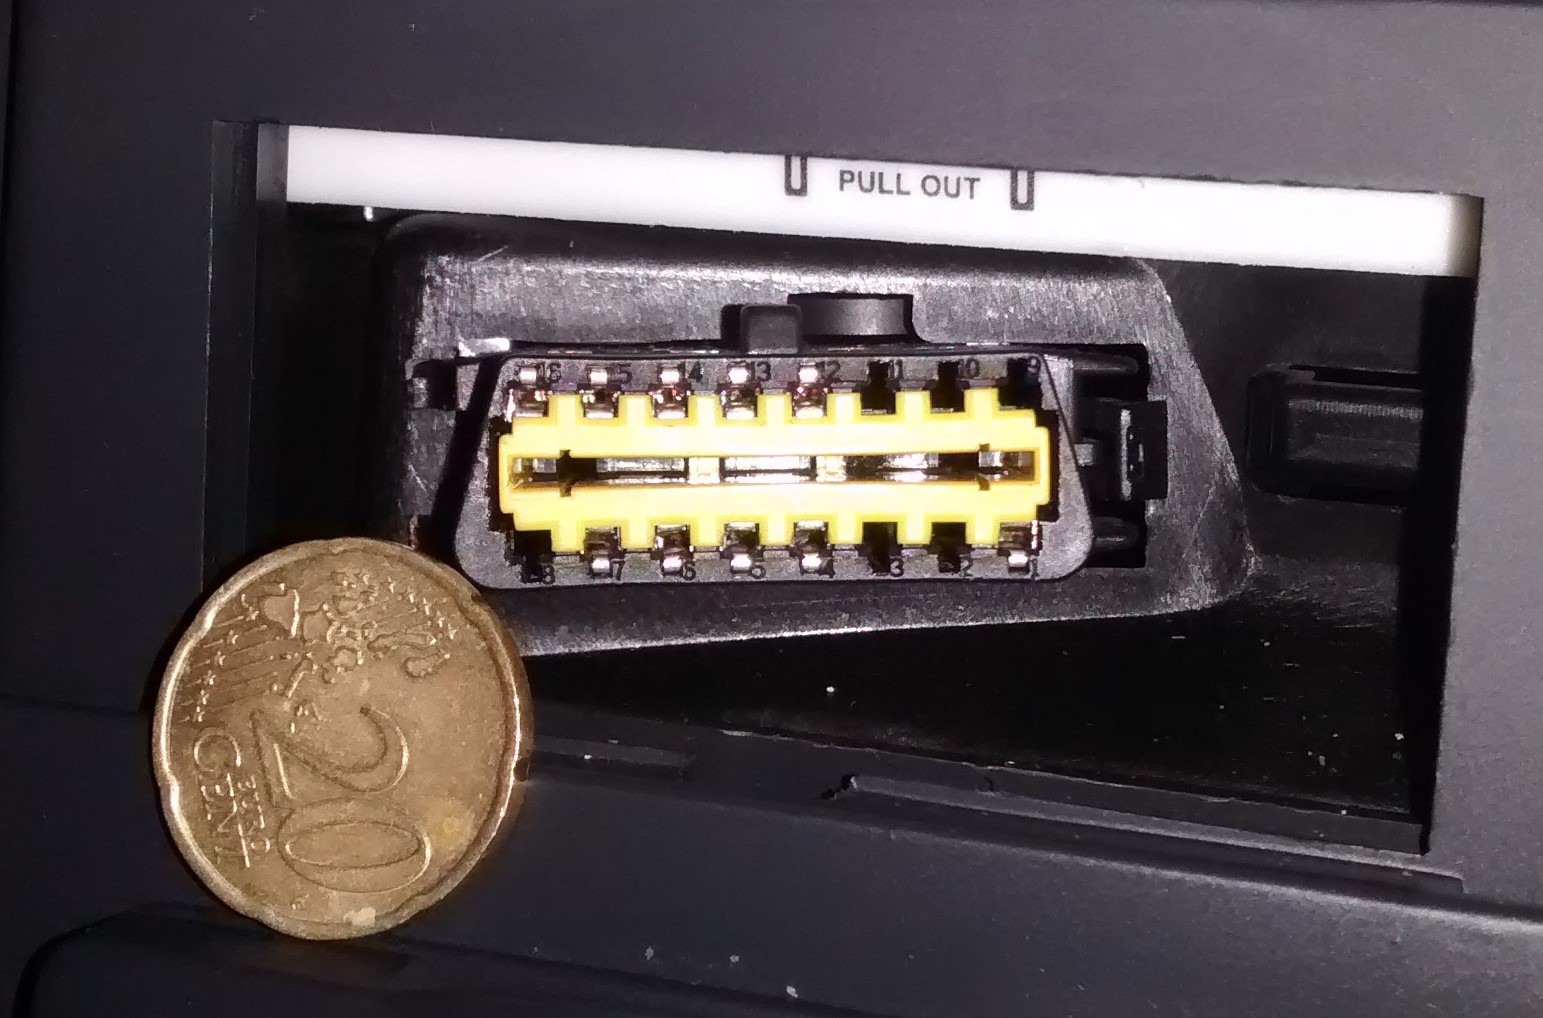
\includegraphics[width=\textwidth]{OBD.jpg}
				\caption{OBDII Port}						
			\end{minipage}
			\hfill			
			\begin{minipage}{0.39\textwidth}
				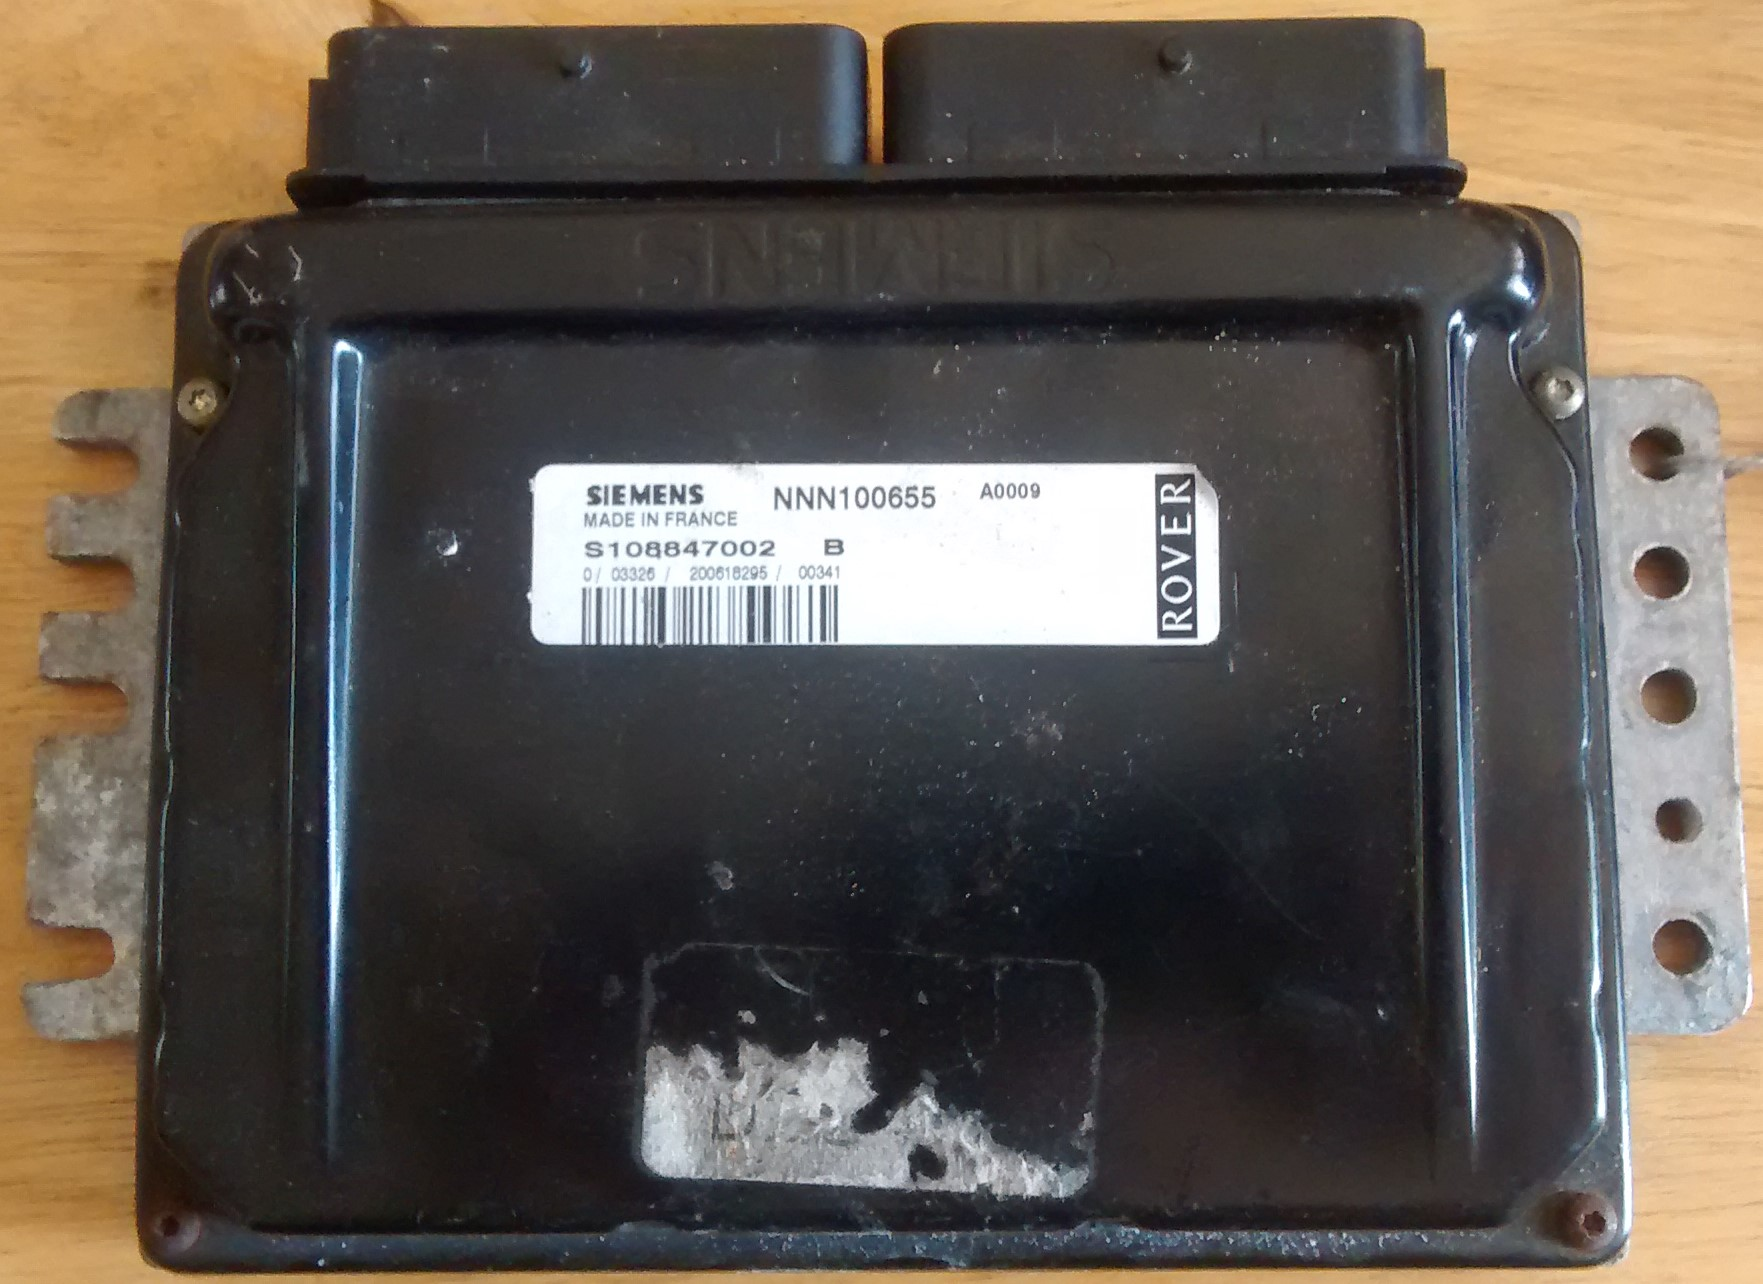
\includegraphics[width=\textwidth]{ECU.jpg}
				\caption{ECU}						
			\end{minipage}									
		\end{center}
	\end{figure}	
\newpage
\section{OBD Communication}
	\subsection{History}{
		\paragraph{}{
		Due to heavy smog pollution in California, CARB introduced regulations requiring all 1988 and newer vehicles sold in California to be fitted with a system for monitoring the emissions of the vehicle. Unfortunately, this system, later named OBDI, had its shortcomings. While new vehicles allowed for monitoring via diagnostic scan tools, the connection port and its position as well as the communication protocols were not standardized, meaning only proprietary scan tools could be used for diagnosis.
		}
		\paragraph{}{
		Prior to the introduction of OBDI, the SAE had proposed a standardised connection port and communication protocols. These changes were taken on board by CARB, and were introduced in OBDII, which was put in force in 1996 in the US. This new system, with it's standardised communication system allowed for generic scan tools to monitor for the vehicle, rather than just proprietary tools.  
		}	
		\paragraph{}{
		Eventually, these regulations reached Europe and Euopean on board diagnostics (EOBD) was introduced. These regulations state that all petrols cars sold in Europe since 2001 and all diesel cars sold in Europe since 2003 must support EOBD. It should be noted that EOBD is the same as OBDII from a technical standpoint.
		}
		\paragraph{}{
		In 2008, regulations were introduced stating that all cars sold in the US must use the ISO 15765 Control Area Network (CAN) communication protocol. A communication protocol defines how data is transferred from the vehicle to the scan tool. This regulation will establish a standard method of communication for all future vehicles.
		}
	}	
	\subsection{Protocols}{
		\paragraph{}{
		The OBDII standards were lenient on how data is transmitted from the vehicle to the scan tool. This lead to vehicle manufacturers creating what they felt was the best way to handle communication. There are now five main communication protocols for OBDII systems.
		\begin{table}[h]
			\begin{center}				
				\begin{tabular}{| l | l |}
				\hline
				\textbf{Protocol} & \textbf{Manufacturer(s)}\\
				\hline
				J1850 Pulse Width Modulation (PWM) & Ford\\
				\hline
				J1850 Variable Pulse Width (VPW) & General Motors\\
				\hline
				ISO 9141-2 & Volkswagen, Audi\\
				\hline
				ISO 14230 Keyword Protocol 2000 (KWP2000) & Chrysler\\
				\hline
				ISO 15765 Control Area Network (CAN) & Toyota\\
				\hline			
				\end{tabular}
				\caption{OBD Protocols}
			\end{center}
		\end{table}	
		}		
		\paragraph{}{
		Regardless of which protocol a vehicle uses, the process for requesting data is the same. The communication process is handled in hexadecimal format, and starts by selecting a mode. A mode represents a specific function to perform and there are ten in total from 01 to 0A. Some modes require a parameter identifier (PID) to be passed, specifying the data item to retrieve. The ECU will send back a response and will have a different conversion method depending on the mode selected. The response will begin with the sum of the mode and $40 _{16}$, for example, if the user requested mode 03, the response would begin with 43.
		}
		\begin{table}[h]
			\begin{center}				
				\begin{tabular}{| l | l |}
				\hline
				\textbf{Mode} & \textbf{Description}\\
				\hline
				01 & Request current powertrain diagnostic data\\
				\hline
				02 & Request powertrain freeze frame data\\
				\hline
				03 & Request emission-related diagnostic trouble codes\\
				\hline
				04 & Clear/Reset emission-related diagnostic information\\
				\hline
				05 & Request oxygen sensor monitoring test results\\
				\hline
				06 & Request on-board sensor monitoring test results\\
				\hline
				07 & Request pending emission-related diagnostic trouble codes\\
				\hline
				08 & Request control of on-board system, test or component\\
				\hline
				09 & Request vehicle information\\
				\hline
				0A & Request permanent emission-related diagnostic trouble codes\\
				\hline
				\end{tabular}
				\caption{OBD Modes}
			\end{center}
		\end{table}		 
		
		\paragraph{}{
		Fortunately, most of the differences between these protocols are low level and do not impact how one can retrieve data from a vehicle using the defined commands. However, there are slight variations when using the CAN protocol.
		}
		\paragraph{}{
		 When requesting DTCs using the CAN protocol, response begins with the number of DTCs, followed by the hex values for each DTC. Using the other protocols, the response only contains the hex values for the DTCs. Mode 05 is unavailable using the CAN protocol and mode 06 must be used as an alternative method to access this data.
		}	
	}
	\subsection{Diagnostic Trouble Codes}{
		\paragraph{}{
		Diagnostic Trouble Codes (DTCs) correspond to faults with a vehicle and are responsible for the illumination of the MIL. Each code begins with an alphabetic letter, indicating the system at fault, followed by four digits specifying the fault. These systems are powertrain, chassis, body and network, represented by the characters P, C, B and U respectively. There are a number of standardized codes, but there are also manufacturer specific codes, which cannot be accessed with generic scan tools.
		}
		\paragraph{}{
		There are three types of DTC: stored, pending and permanent, accessed by mode 03, 07 and 0A respectively. Stored codes represent current issues with the vehicle. These codes can sometimes be fixed by calling the clear codes command on the scan tool. Pending codes represent potential future issues. If there is an irregular data value found by a sensor it may create a pending code. The ECU will continue to monitor this sensor, and if the data value has not returned to the expected value after a certain amount of time, the pending code is converted to a stored code. Otherwise, the pending code will be removed automatically. Permanent codes represent serious issues with the vehicle. These codes are not removed manually by scan tools or automatically by the ECU. In order to remove these codes, the underlying issue that caused the code to appear must be fixed.
		}			
	}
	\subsection{Clear Codes}{
		\paragraph{}{
		The clear codes function allows one to clear all emissions-related diagnostic information from the ECU and can be accessed by mode 04. This removes stored and pending DTCs, on-board monitoring test results, oxygen sensor data, freeze frame data and data items pertaining to DTC and MIL information, such as distance travelled while MIL is activated.
		}
		\paragraph{}{
		In some cases, clear codes can turn off the MIL permanently. However, if the underlying issues are still present after the clear codes command has been sent, the MIL will illuminate again.
		}
	}
	
	\subsection{Data}{
		\paragraph{}{
		Emission related data can be accessed via mode 01. This data is retrieved from the sensors and subsystems of the vehicle. In this mode, the user must specify a PID in order to display a certain data item , for example, the PID 0C returns the engine speed.
		}
		\paragraph{}{
		The first step when requesting data is to find the PIDs that are supported for this vehicle, as some vehicles may only support a subset of PIDs. This can be achieved by using PIDs 00, 20, 40, 60 and 80, each of which represent the next 32 PIDs. This will return a hexadecimal value that, when converted to binary, denotes which PIDs are supported. Each bit in the binary string represents a PID. If the bit is 1, the PID is supported and if it is 0 the PID is unsupported.
						
		}
		\paragraph{}{
		As an example, we call 0120, to request the next 32 supported PIDs from 21 to 40. In this example, we receive the hexadecimal response \textit{1A300100}. When this response has been converted to binary, we get the following string: \[0001 1010 0011 0000 0000 0001 0000 0000\] The most significant bit represents PID $21 _{16}$ and the least significant bit represents PID $40 _{16}$. If we look at the bits that are set to one, we determine that PIDs 24, 25, 27, 2B, 2C and 38 are supported.
		}
		\paragraph{}{
		Once the list of supported PIDs has been established, the user can request the data for these PIDs. This will return a single data value, so in order for the scan tool to display live data, it must repeat this call. The response must be converted from hexadecimal to the appropriate human readable value, either a string or number. Each PID has a different conversion method, although some PIDs may share them, for example engine coolant temperature and intake air temperature.
		}
	}
	\subsection{Other Modes}{
		\paragraph{}{
		Mode 02 allows access to freeze frame data. When a DTC is stored, the ECU takes a snapshot of the values for each available data item. This snapshot is known as freeze frame data. It is accessed and converted in the same way as PID data, although each data item only has one value. It can be used to pinpoint which component is at fault by checking for irregular data values.
		}		
		\paragraph{}{
		Mode 05 allows access to oxygen sensor monitoring test results. These sensors monitor the richness of the air/fuel mixture, which may affect the performance and fuel consumption of the vehicle. Mode 05 is no longer supported in the CAN protocol, but the data can be accessed via Mode 06 instead.
		}
		\paragraph{}{
		Mode 06 allows access monitoring test results for specific components, such as catalyst monitoring. It can be used as an alternative to Mode 05 to access oxygen sensor monitoring. The user must pass a specific test identifier that is supported by the ECU. The method of finding the supported test identifiers is similar to the process of finding supported PIDs in Mode 02. 
		}
		\paragraph{}{
		Mode 09 allows access to vehicle information. The information available depends on the vehicle, but every vehicle has a vehicle identification number (VIN). This is a 17 character identifier unique to that vehicle, which can be used to search for the history of the vehicle. 
		}
	}

\section{Technology}
	\subsection{ELM327}{}{
		\paragraph{}{
		The ELM327 device I will use for this project is a compact and inexpensive Bluetooth dongle that can connect to the OBDII port on modern vehicles. It supports all OBDII protocols and abstracts the data transfer process by including its own set of commands to handle communication.				
		}
		\paragraph{}{
		The commands that the device supports allow users to either manually or automatically select the protocol, depending on if they know which protocol their vehicle uses. These commands also handle initialization of the device, setting up communication, and formatting the data received from the vehicle. Once the device has been configured, the user can send requests to the vehicle. These requests are in the same format that they are found in the SAE J1979 document, and no further formatting is required.
		}
		\paragraph{}{
		The ELM327 device is easy to set up, without any technical knowledge. The communication set up is handled by the application that it is connected to, so the end user only has to connect the device to the vehicle and the computer or device that the application runs on. The device is also relatively inexpensive and easy to find on well known retail sites such as Amazon, so it is readily available for users who may not know of specialist retailers for diagnostic scan tools.
		}
		\begin{figure}[h]
				\begin{center}											
					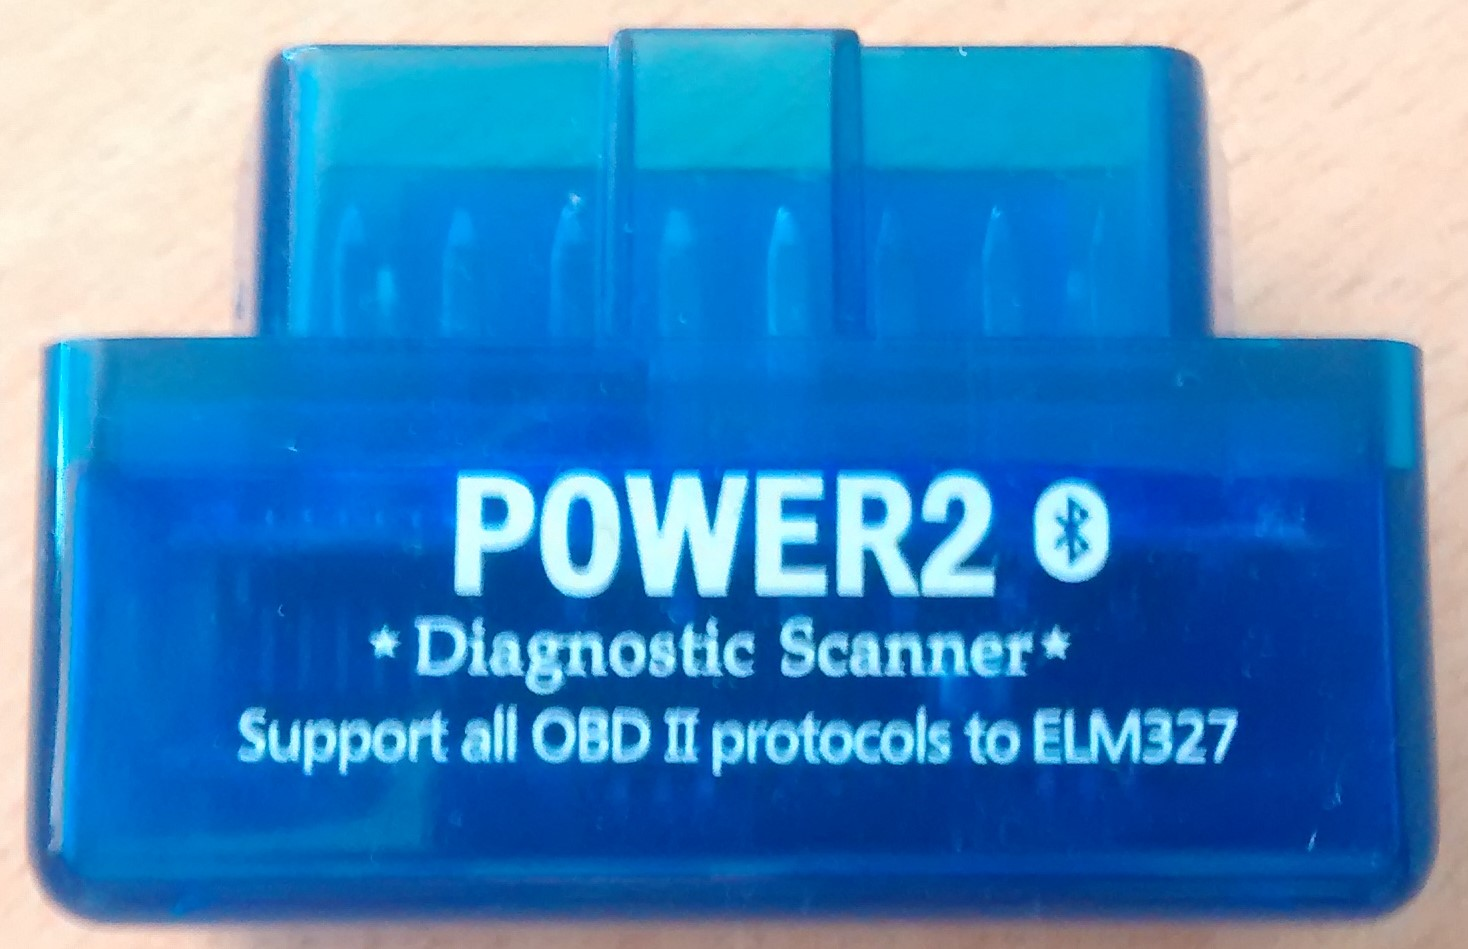
\includegraphics[width=0.4\textwidth]{ELM327.jpg}
					\caption{ELM327 Bluetooth Dongle}											
				\end{center}
			\end{figure}		
	}	
	\subsection{Windows 10}{}{
		\paragraph{}{
		}	
	}
	\subsection{Xamarin}{
		\paragraph{}{
		}	
	}

\section{Similar Applications}
	\paragraph{}{
	When looking at similar applications, I opted to look at applications developed using the same technology and deployed on the same platform that I intended to use. This lead me to find two similar applications available on Windows 10 through the Windows Store. I investigated what modes these applications included, their communication process, the hardware required and the general look and feel of the user interface.
	}
	\subsection{Diagnose your car}
		\paragraph{}{
		Modes included, Connection, UI etc
		}
	\subsection{OBDdash}
		\paragraph{}{
		Modes included, Connection, UI etc
		}	
	
\section{Architectural Patterns}
	\paragraph{Intro}{
	}	
	\paragraph{MVVM}{
	}